%!TEX root = ../main.tex
\section{Cơ sở lý thuyết}

\subsection{Thuật toán tiến hóa đa nhiệm}

\begin{frame}{Thuật toán tiến hóa đa nhiệm - 1}
    \begin{alertblock}{Phát biểu bài toán}
        \begin{itemize}
            \item \textbf{Cho:} $K$ bài toán tối ưu.
            \item Tác vụ $T_k$ ứng với việc giải bài toán thứ $k$.
            \item $T_k$ có không gian tìm kiếm $\mathcal{X}_k$, hàm mục tiêu $f_k:\mathcal{X}_k \rightarrow \mathbb{R}$
            \item \textbf{Yêu cầu:} tìm $\{x^*_1, x^*_2, \ldots, x^*_{K-1}, x^*_K\}=argmin\{f_1(x), f_2(x), \ldots, f_{K-1}(x), f_K(x)\}$ với $x^*_k$ là nghiệm tối ưu toàn cục của $T_k$.
        \end{itemize}
    \end{alertblock}
    \begin{block}{Tính chất đặt biệt của tiến hóa đa nhiệm}
        Việc giải tác vụ $T_k$ có thể có ảnh hưởng tốt giúp giải $T_{k'}, k' \ne k$ tối ưu hơn.
    \end{block}
\end{frame}

\begin{frame}{Thuật toán tiến hóa đa nhiệm - 2}
    \begin{alertblock}{Không gian biểu diễn chung}
        \begin{itemize}
            \item \textbf{Cho:} $K$ tác vụ với chiều lần lượt là $\{D_1, D_2, \ldots, D_{K}\}$.
            \item \textbf{Biểu diễn chung:} $D_{unified}=max\{D_1, D_2, \ldots, D_{K}\}$.
        \end{itemize}
    \end{alertblock}
    \begin{alertblock}{Không gian biểu diễn chung trong tối ưu số thực}
        \begin{itemize}
            \item Quy ước là $[0, 1]^{D_{unified}}$.
        \end{itemize}
    \end{alertblock}
    \begin{block}{Cách sử dụng không gian biểu diễn chung}
        \begin{itemize}
            \item Thực hiện toán tử tiến hóa trên cá thể với chiều $D_{unified}$.
            \item Đánh giá trên cá thể với chiều $\{D_1, D_2, \ldots, D_{K}\}$.
        \end{itemize}
    \end{block}
\end{frame}

\begin{frame}{Thuật toán tiến hóa đa nhiệm - 3}
    \begin{columns}
        \begin{column}{0.45\textwidth}
            \begin{block}{MFEA - Multifactorial Evolutionary Algorithm}
                \begin{figure}
                    \centering
                    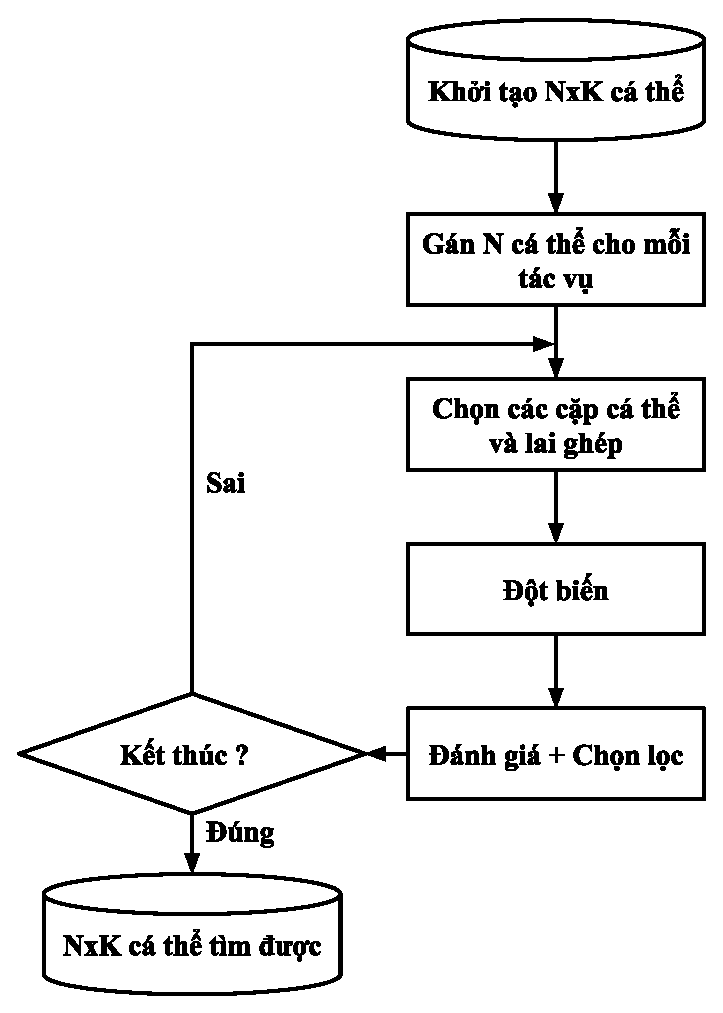
\includegraphics[width=0.7\linewidth]{figure/preliminary/mfea.eps}
                    \caption{Khung thuật toán MFEA}
                    \label{fig:preliminary:mfea}
                \end{figure}
            \end{block}
        \end{column}
        \begin{column}{0.45\textwidth}
            \begin{alertblock}{Skill factor}
                \fontsize{6pt}{10}\selectfont
                \emph{Skill factor} $\tau_i$ của cá thể $i^{th}$ là index của tác vụ trong $K$ tác vụ, mà cá thể $i$ thuộc về.
            \end{alertblock}
            \begin{algorithm}[H]
                \fontsize{6pt}{10}\selectfont
                \caption{\fontsize{6pt}{10}\selectfont Lai ghép trong MFEA}
                \begin{algorithmic}[1]
                    \State Lấy ngẫu nhiên hai cá thể cha mẹ $p_a$ và $p_b$ từ $P$
                    \If{$\tau_a == \tau_b$}
                        \State $[c_a, c_b] \leftarrow$ \emph{Lai ghép cùng tác vụ} giữa $p_a$ và $p_b$
                        \State Gán \emph{skill factor} $\tau_a$ cho $c_a$ và $c_b$
                    \ElsIf{{\color{red}$rand \le rmp$}}
                        \State {\color{red}$[c_a, c_b] \leftarrow$ \emph{Lai ghép khác tác vụ} giữa $p_a$ và $p_b$}
                        \State Gãn ngẫu nhiên \emph{skill factor} $\tau_a$ or $\tau_b$ cho từng con sinh ra
                    \Else
                        \State Gán \emph{skill factor} $\tau_a$ cho $c_a$ 
                        \State Gán \emph{skill factor} $\tau_b$ cho $c_b$
                    \EndIf
                \end{algorithmic}
                \label{alg:preliminary:mfea}
            \end{algorithm}
        \end{column}
    \end{columns}
\end{frame}

\subsection{Mô hình Multi-Armed Bandits}

\begin{frame}{Mô hình Multi-Armed Bandits - 1}
    \begin{columns}
        \begin{column}{0.45\textwidth}
            \begin{block}{Nguồn gốc tên gọi Multi-Armed Bandits}
                \begin{figure}
                    \centering
                    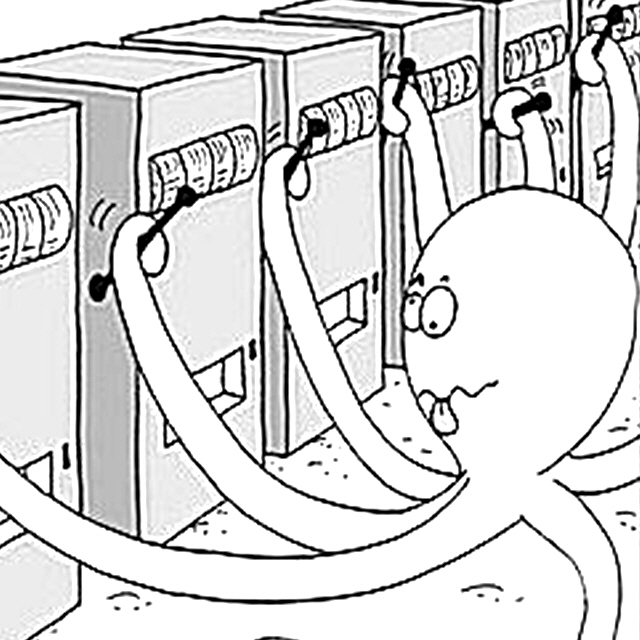
\includegraphics[width=0.7\linewidth]{figure/preliminary/multi-armed-octopus.jpg}
                    \caption{Lựa chọn chơi máy nào, thứ tự thế nào, mỗi máy bao lần, thắng càng nhiều tiền càng tốt}
                    \label{fig:preliminary:mab}
                \end{figure}
            \end{block}
        \end{column}
        \begin{column}{0.45\textwidth}
            \begin{algorithm}[H]
                \fontsize{8pt}{10}\selectfont
                \caption{\fontsize{8pt}{10}\selectfont Mô hình Multi-armed bandits}
                \begin{algorithmic}[1]
                    \\
                    \textbf{Cho:} $K$ lựa chọn, $T$ vòng.
                    \For{vòng thứ $t \in \{1, \ldots, T\}$}
                        \State Chọn lựa chọn $a_t$;
                        \State Nhận về phần thưởng $r_t \in [0, 1]$ cho lựa chọn $a_t$;
                    \EndFor
                \end{algorithmic}
                \label{alg:preliminary:mab}
            \end{algorithm}
        \end{column}
    \end{columns}
    % The name comes from imagining a gambler at a row of slot machines (sometimes known as "one-armed bandits"), who has to decide which machines to play, how many times to play each machine and in which order to play them, and whether to continue with the current machine or try a different machine.
\end{frame}

\begin{frame}{Mô hình Multi-Armed Bandits - 2}
    \begin{block}{Ứng dụng của MAB}
        \begin{columns}
            \begin{column}{0.45\textwidth}
                \begin{figure}
                    \centering
                    
\includegraphics[width=0.7\linewidth]{figure/preliminary/news.eps}
                    \caption{Lựa chọn nguồn in và đề xuất tin tức sao cho người dùng xem nhiều nhất}
                    \label{fig:preliminary:news}
                \end{figure}
            \end{column}
            \begin{column}{0.45\textwidth}
                \begin{figure}
                    \centering
                    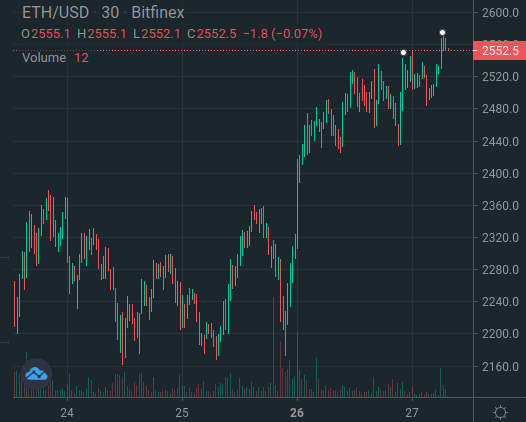
\includegraphics[width=0.7\linewidth]{figure/preliminary/eth-usd.png}
                    \caption{Lựa chọn kênh đầu tư sao cho lãi nhất}
                    \label{fig:preliminary:invest}
                \end{figure}
            \end{column}
        \end{columns}
    \end{block}
\end{frame}
